\RequirePackage{luatex85}
\documentclass{standalone}

\usepackage{amsmath}

\usepackage{fontspec, unicode-math}
\setsansfont[Scale=MatchLowercase]{TeX Gyre Heros}
\setmathfont{TeX Gyre Termes Math}

\usepackage{tikz}
\usepackage{pgfplots}
\pgfplotsset{compat=1.14}

\tikzset{
  every picture/.style={font={\sffamily\normalsize}, >=stealth},
  every pin edge/.style={black}}

\begin{document}

  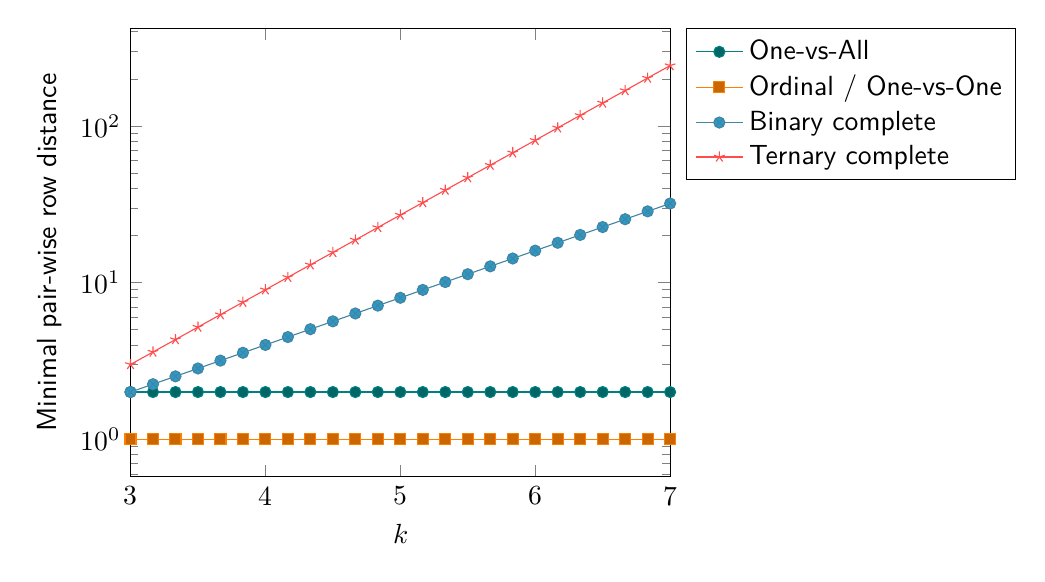
\begin{tikzpicture}
    \begin{semilogyaxis}[xmin=3, xmax=7, ymin=0, domain=3:7,
      legend pos=outer north east, legend cell align=left, cycle list name={exotic},
      ylabel={Minimal pair-wise row distance}, xlabel={$k$}]

      \addplot {2};
      \addlegendentry{One-vs-All};

      \addplot {1};
      \addlegendentry{Ordinal / One-vs-One};

      \addplot {2^(x-2)};
      \addlegendentry{Binary complete};

      \addplot {(3^(x-2)};
      \addlegendentry{Ternary complete};
    \end{semilogyaxis}
  \end{tikzpicture}

\end{document}
